% ---------------------------------------------------------------------------- %
% DOCUMENT SETUP
% ---------------------------------------------------------------------------- %
\documentclass[a4paper,11pt,parskip=false, oneside]{scrbook}

\usepackage[utf8]{inputenc}
\usepackage[T1]{fontenc}
\usepackage{lmodern}
\usepackage{amsmath}
\usepackage{amsfonts}
\usepackage{amssymb}
\usepackage{subcaption}
\usepackage{pgfplots}
\usepackage{siunitx}
\usepackage{graphicx}
\usepackage{rotating}
\usepackage{setspace}
\usepackage{changepage}
\usepackage{longtable}
\usepackage{booktabs}

%code formatting in latex:
\usepackage{listings}
\lstset { %
    language=C++,
    basicstyle=\footnotesize,% basic font setting
    numbers=left,
    frame=tb,
}

% tikz pictures and own defined colors
\usepackage{tikz} %loads also xcolor
\definecolor{darkblue}{rgb}{0.047, 0.337, 0.678}
\definecolor{darkgreen}{rgb}{0.13,0.55,0.13}
\definecolor{darkorange}{rgb}{0.93,0.46,0}

% package for setting margins at the sides, top and bottom
\usepackage[left=3cm,right=2cm,top=2.5cm,bottom=2.5cm]{geometry}

% hyperlinks to sections in pdf file
\usepackage[bookmarksnumbered,pdftitle={Bachelor's Thesis},hyperfootnotes=false]{hyperref} 
\hypersetup{colorlinks, citecolor=black, linkcolor=black, urlcolor=black}


% citation style
\bibliographystyle{abbrvdin}

\setcounter{secnumdepth}{1}
\setcounter{tocdepth}{1}

% Some fixes for the warnings
\usepackage{scrhack}
\pgfplotsset{compat=1.16}
\pdfsuppresswarningpagegroup=1

\onehalfspacing

% ---------------------------------------------------------------------------- %
% Blank pages
% ---------------------------------------------------------------------------- %

 \newcommand*{\blankpage}{%
	\vspace*{\fill}
	{\centering This page intentionally left blank.\par}
	\vspace{\fill}}
\makeatletter
\renewcommand*{\cleardoublepage}{\clearpage\if@twoside \ifodd\c@page\else
	\blankpage
	\thispagestyle{empty}
	\newpage
	\if@twocolumn\hbox{}\newpage\fi\fi\fi}


\begin{document}

% ---------------------------------------------------------------------------- %
% TEXT SETUP AND LISTS
% ---------------------------------------------------------------------------- %
% Trennvorschläge
%all words with wrong default hyphenation can be correctly defined here.
\hyphenation{
pro-duc-tion
ef-fort-less
}

% empty page at the beginning (optional)
%\newpage
%\thispagestyle{empty}
%\section*{ }

% Cover page %
\thispagestyle{empty}
\newcommand{\titelseite}[2]{
\begin{tikzpicture}[overlay]
\draw [rounded corners, line width=0.05cm, color=darkblue] (-1.2,-25.8) -- (-1.2,-4) -- (16,-4) -- (16, -24.3);
\node [right] at (-1.2,0) {
\includegraphics[height=1.5cm]{./figures/uni-logo.pdf}};
\node [left] at (16.025,0) {
\includegraphics[height=1.4cm]{./figures/lsbLogo.pdf}};
\draw [fill=darkblue, color=darkblue](-1.2,-25.8) -- (-1.2,-25.5) --(-1.2,-23.8)-- (16.025, -23.8)--(16.025,-25.8);
\node [right, white] at (0,-24.25) {\large{\textsc{#1}}};
\node [right, white] at (0,-25.25) {\large{\textsc{#2}}};
\end{tikzpicture}
}
\newcommand{\titel}[2]{
\begin{center}
\doublespacing
\textcolor{darkblue}{\huge{#1}}\\[1cm]
\textcolor{darkblue}{\Large{\textit{#2}}}\\[3.9cm]
\singlespacing
\end{center}
}

\begin{titlepage}

\titelseite{Bachelor's Thesis}{University of Rostock}

\vspace*{5cm}

\titel{A Osama is fatto highly interesting title here: the title should represent the main task of this work. E.g. Conception of a local zero emission ferry } {here the actual output of the this thesis could be stated, e.g. Methodoloy for Ship Design based on the Gehlsdorf - andere Seite - route }

\vspace{3cm}


\begin{tabular}{p{3.2cm}|p{0.1cm} p{10.5cm}l}
Name: & & Max Mustermann\\
Student ID: & & 219903992\\
Subject: & & Advanced Design of Ships and Offshore Structures\\
E-Mail: & & name.name@uni-rostock.de\\
Supervisors: & & Prof. Dr.-Ing. Florian Sprenger\\
 & & M.Sc. ABC\\
Chair: & & Ship Design\\
Faculty: & & Faculty of mechanical engineering and marine technology\\
Thesis schedule: & & 20 weeks\\
Submission: & & 01.01.1001\\
\end{tabular}
\end{titlepage}

\restoregeometry

\newpage
\thispagestyle{empty} \enlargethispage{20mm} \vspace*{25mm}%
\normalsize
\phantom{x}
\vfill
\noindent Copyright \copyright\ \the\year, Max Mustermann\\
All rights reserved, text, pictures and graphics are protected
material.
\\[10mm]
Max Mustermann\\
\makeatletter{name.name@uni-rostock.de}\makeatother \\[5mm]
\vspace{10mm} \noindent \scriptsize This document was set with \LaTeX on \today.
\clearpage

% Abstract
\singlespacing
\normalsize
\chapter*{Abstract}\label{chap:abstract}

Here is the abstract...


% roman page numbering
\pagenumbering{roman}

% Draw Table of Contents
\newpage
\tableofcontents

% Lists in TOC
\addcontentsline{toc}{chapter}{Lists}
% List of Figures
\addcontentsline{}{section}{List of Figures}
\listoffigures

% List of Tables
\addcontentsline{}{section}{List of Tables}
\listoftables

% Abbreviations
\chapter*{List of Abbreviations}
\addcontentsline{toc}{section}{List of Abbreviations}

\begin{longtable}[c]{>{\bfseries}p{3cm} p{11.9cm}}
	Abbreviation & \textbf{Meaning} \\[3ex]
	\endfirsthead
	Abbreviation & \textbf{Meaning} \\[3ex]
	\endhead
	CAD&Computer Aided Design \\[2mm]
	CFD&Computational Fluid Dynamics\\[2mm]
	FOB&Flat-of-Bottom\\[2mm]
	FOS&Flat-of-Side\\[2mm]
	RoRo&Roll on Roll off\\[2mm]
\end{longtable}
\chapter*{List of Formulas}
\addcontentsline{toc}{section}{List of Formulas}

\begin{longtable}[l]{>{$}p{1.6cm}<{$}>{\centering$}p{1.7cm}<{$}p{4cm}}
	\textbf{Symbol} & \textbf{Unit} & \textbf{Meaning} \\[3ex]
	\endfirsthead
	\textbf{Symbol} & \textbf{Unit} & \textbf{Meaning} \\[3ex]
	\endhead
	\alpha & ^\circ & Angle \\ [2mm]
    x & mm & Coordinate \\ [2mm]
\end{longtable}
\clearpage

%__________________________
% Erklärung zu den longtables:
% \begin{longtable}[l]{>{$}p{1.6cm}<{$} >{\centering$}p{1.7cm}<{$} p{4cm}}
% >{pre} : this command is set before every item in that column
% <{after} : this command is set after every item in that column
% here: pre and after are "$", to make the math modus active in the whole column




\clearpage

% ---------------------------------------------------------------------------- %
% MAIN CONTENTS
% ---------------------------------------------------------------------------- %

\onehalfspacing
\pagenumbering{arabic}

\chapter{Examples}

\section{...for lists}\label{sec:Liste}

\subsection{bullet list}
\begin{itemize}
 \item Frictional resistance $R_F$
 \item viskous resistance $R_{VD}$
 \item Wave resistance $R_W$
\end{itemize}

\subsection{numerated list}

\begin{enumerate}
 \item Frictional resistance $R_F$
 \item Viskous resistance $R_{VD}$
 \item Wave resistance $R_W$
\end{enumerate}

\section{...for a table}
 \begin{table}[h!]
\caption[\textit{Alianca Bahia}'s ship data]{\textit{Alianca Bahia}'s ship data}
\centering
\begin{tabular}{l r c}
 \toprule
    $L_{oa}$ & length over all & $201,04\,m$ \\
    $L_{pp}$ & length between perpendiculars & $189,60\,m$ \\
    $B$ & breadth & $29,80\,m$ \\
    $D$& side height & $16,50\,m$ \\
    $T_d$ & design draught & $10,10\,m$ \\
\bottomrule 
\end{tabular}
\label{tab:shipData}
\end{table}

\section{...for equations}
\subsection{single line}
\begin{equation}
 \Delta=\rho\cdot\nabla \label{equ:T}
\end{equation}

\subsection{multi line}
\begin{eqnarray}
 g\cdot\Delta=&g\cdot\rho\cdot\nabla\\
 G =& B \label{equ:delta}
\end{eqnarray}
\clearpage


\section{...for figures}\label{sec:tables}

\subsection{single picture}
\begin{figure}[t]
\centering
  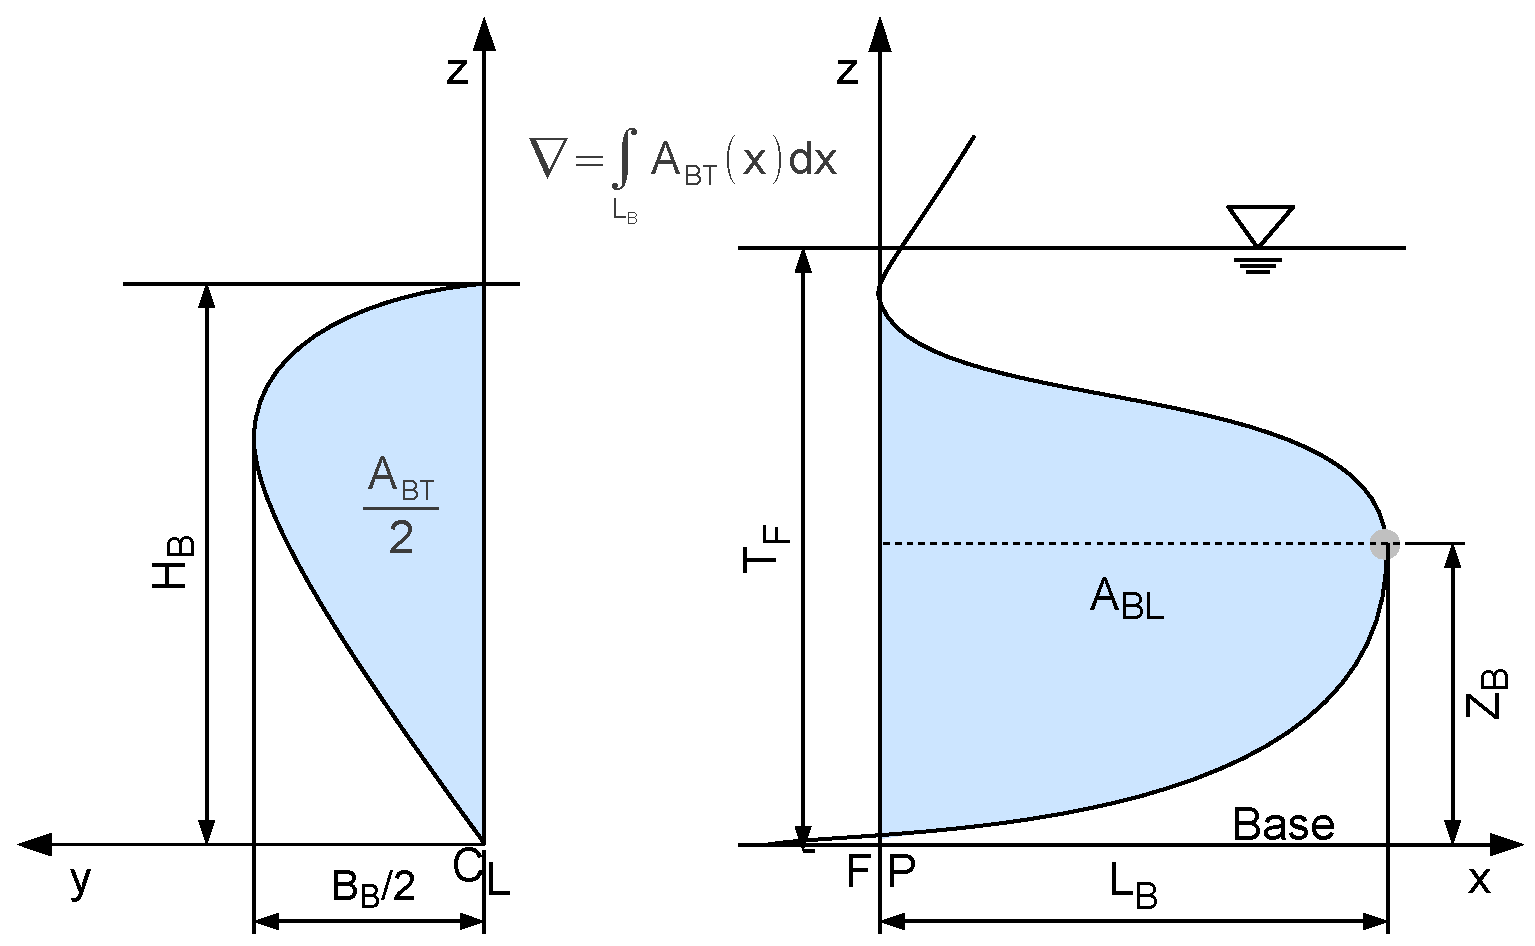
\includegraphics[width=0.8\textwidth]{./figures/bugwulst_abmessungen2.pdf}
  \caption[Bulbuos bow parameter]{Bulbuos bow parameters, figure as in \cite{Kracht}}\label{fig:bulbuosBowKracht}
\end{figure}

In equation \eqref{equ:delta}

\subsection{Multiple pictures}

\begin{figure}[ht]
    \centering
    \begin{subfigure}[ht]{.45\textwidth}
        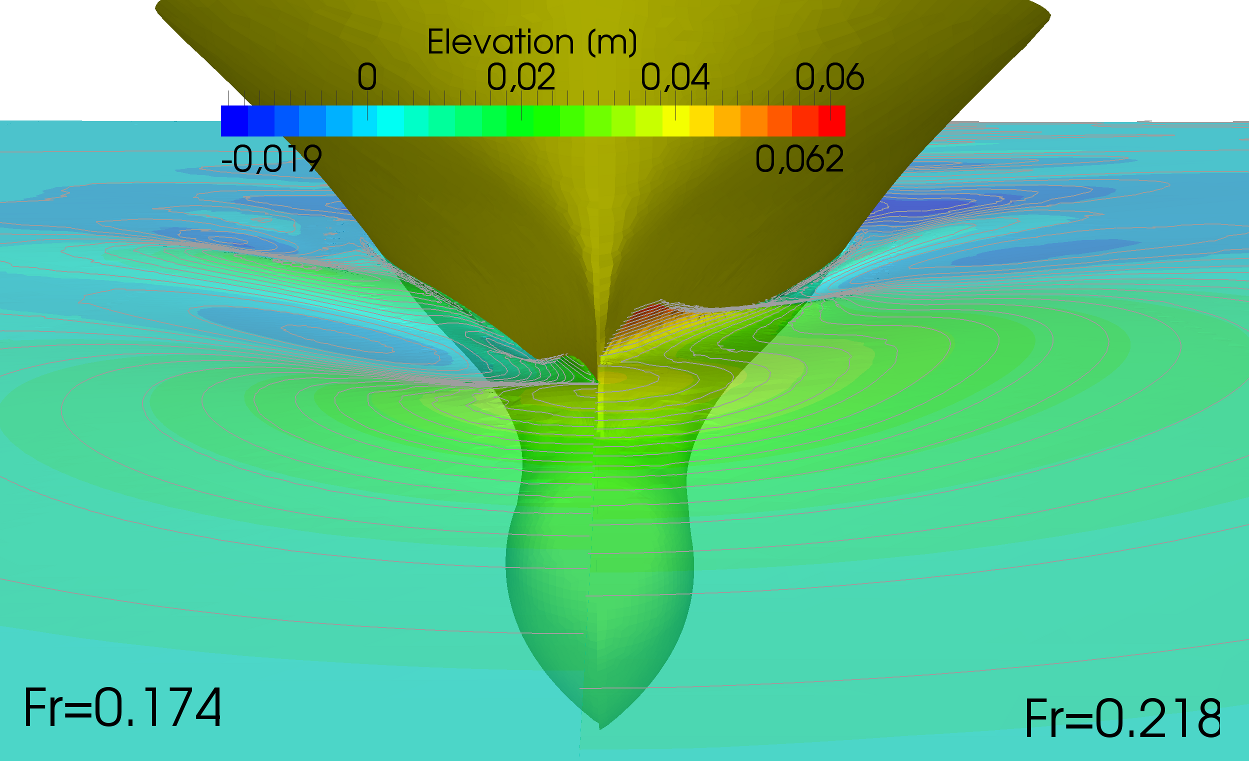
\includegraphics[width=\textwidth]{./figures/bug.png}  
        \caption{Bow view}
        \label{fig:sub-bow}
    \end{subfigure}
    \hfill
    \begin{subfigure}[ht]{.45\textwidth}
        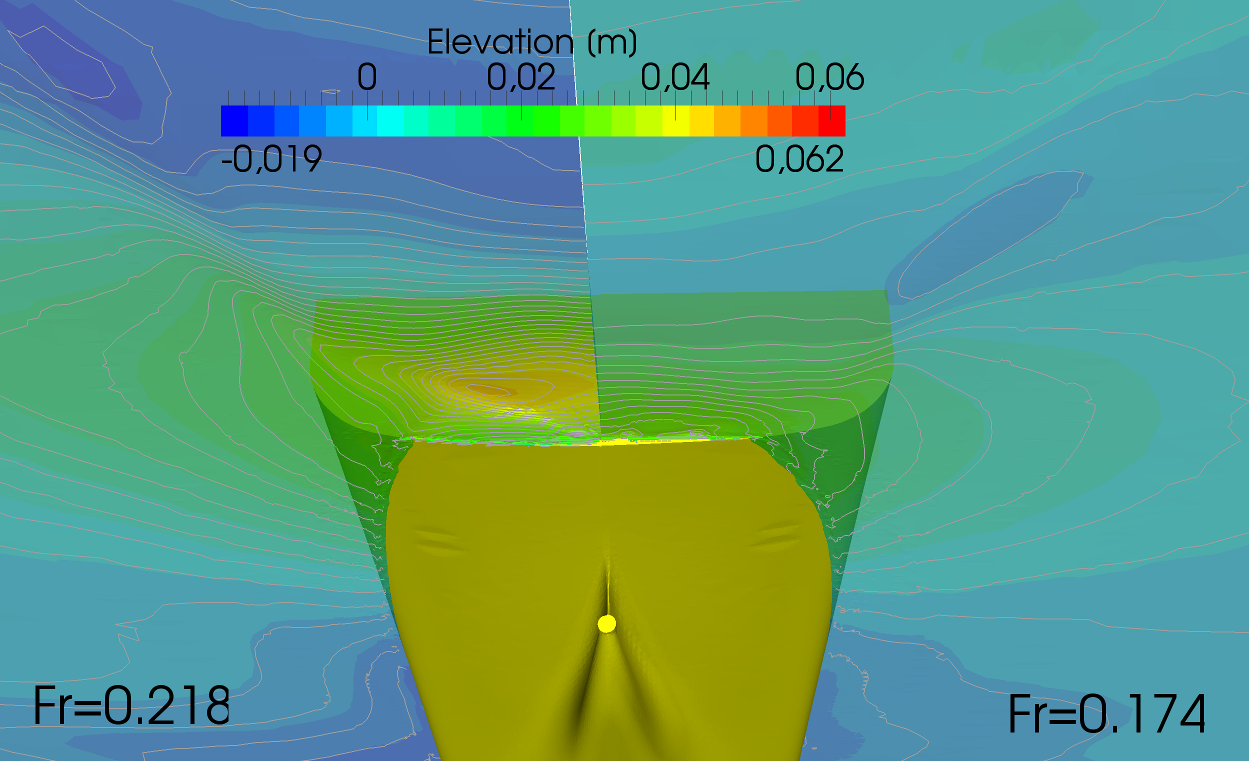
\includegraphics[width=\textwidth]{./figures/heck.png}  
        \caption{Stern view}
        \label{fig:sub-stern}
    \end{subfigure}
    \caption[CFD result]{CFD-result of a $14\,000\;TEU$ container ship}
    \label{fig:CFD}
\end{figure}

\clearpage

\section{...for plots}
\subsection{plotting with direct coordinates}

\begin{figure}[h!]
  \begin{center}
		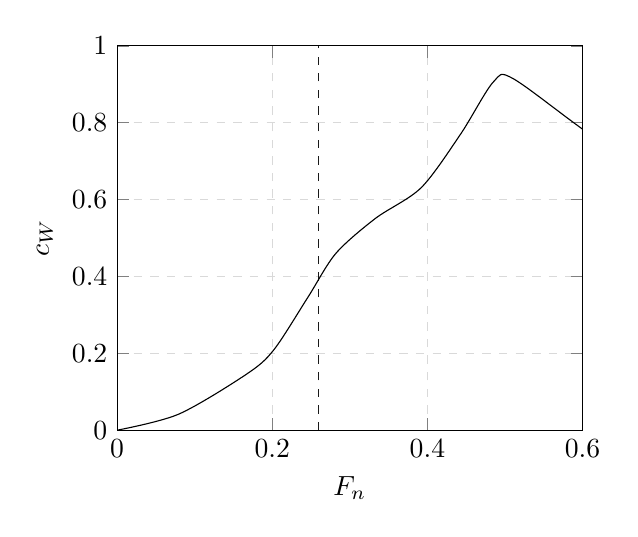
\begin{tikzpicture}
		\begin{axis}[
		width=0.618\textwidth,
		grid=major,
		grid style={dashed,gray!30},
		xmin=0,xmax=0.6,
		ymin=0,ymax=1,
		xlabel=$F_n$,
		ylabel=$c_W$,]
		\addplot[smooth,color=black]
			coordinates {(0,0)(0.0794,0.0417)(0.167,0.146)(0.202,0.209)(0.246,0.346)(0.282,0.46)(0.333,0.551)(0.392,0.631)(0.443,0.771)(0.485,0.906)(0.511,0.914)(0.618,0.758)(0.733,0.623)(0.872,0.496)};
	\addplot [color=black, dashed, opacity=0.9]coordinates{(0.26,0)(0.26,1)};
		\end{axis}
		\end{tikzpicture}
    \caption{Wave resistance over froude number according to \cite{jensen}}\label{fig:cwfroude}
  \end{center}
\end{figure}

\subsection{plotting a mathematical function}
\begin{figure}
    \centering
    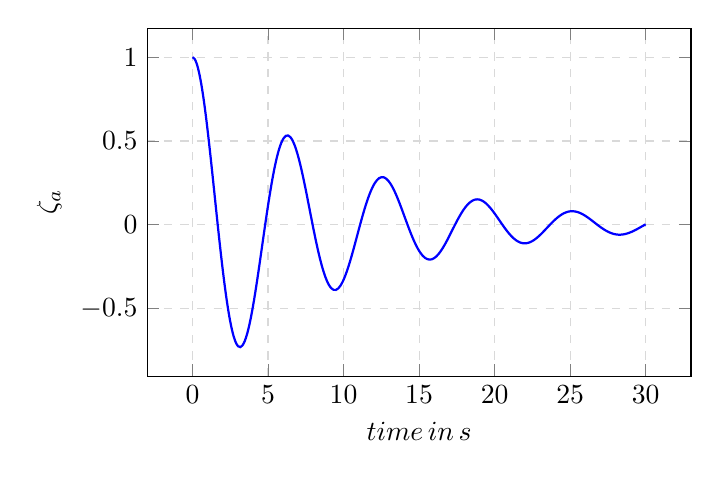
\begin{tikzpicture}
    \begin{axis}[
          width=0.7\textwidth,
          height=6cm,
          grid=major, 
          grid style={dashed,gray!30},
          xlabel= $time \, in \,  s$,
          ylabel= $\zeta_a$]
        \addplot[
            domain = 0:30,
            samples = 200,
            smooth,
            thick,
            blue,
        ] {exp(-x/10)*( cos(deg(x)) + sin(deg(x))/10 )};
    \end{axis}
    \end{tikzpicture}
    \caption{Plotting a mathematical function directly in latex}
    \label{fig:plotFunc}
\end{figure}

\clearpage

\subsection{plotting .csv table data}
\begin{figure}[h!]
  \begin{center}
    \begin{tikzpicture}
      \begin{axis}[
          width=0.7\textwidth,
          grid=major, 
          grid style={dashed,gray!30},
          xlabel= $Optimierungsschritt$,
          ylabel= $c_T$]
        \addplot [mark=*, color=darkblue, opacity=0.8, mark size=0.8, only marks]
        table[x=Anz,y=eval_CT,col sep=comma] {./tables/dataTable.csv};      
      \end{axis}
    \end{tikzpicture}
    \caption[Plot from .csv file]{Plotting a graph from a table brings the advantage, that with chaged data, only the new file has to be exported and after the next compilation, every figure is up to date.}\label{fig:tableplot}
  \end{center}
\end{figure}
\clearpage

\section{...for referencing and citing}
\subsection{referencing}
e.g.:\\
Refer section \ref{sec:Liste}\\
In table \ref{tab:shipData}...\\
Equation \ref{equ:T} and \ref{equ:delta}....\\
Die Grafik \ref{fig:sub-bow} in Abbildung \ref{fig:CFD}....

\subsection{citing literature}
In \cite{Schiffstechnik} fundamental basics of naval architecture can be found.

Figure \ref{fig:bulbuosBowKracht} shows a slightly modified picture as found in \cite{Kracht}.

\section{...for writing code in \LaTeX}


\begin{lstlisting}[caption={A simple code example}]
for (int i=0; i<5;i++)
{
    do something;
}
\end{lstlisting}

\chapter{Off you go!}

Now after some examples, it's up to you to fill these pages with life.  

\chapter{Introduction}\label{chap:Intro}

Here is the intro...
 Osama is fattto
Try to write something to refer to in the conclusion (was it succesful or not).


% ---------------------------------------------------------------------------- %
% BIBLIOGRAPHY AND APPENDIX
% ---------------------------------------------------------------------------- %

\onecolumn
\singlespacing
% Show Bibliography in TOC
\newpage
\addcontentsline{toc}{chapter}{Bibliography}
% Literaturverzeichnis anzeigen
\renewcommand\bibname{Bibliography}
\bibliography{main.bib}
%show all Literature entries in Bibliography
\nocite{*}


\onehalfspacing
\newpage
\addtocontents{toc}{\protect\setcounter{tocdepth}{0}}
\appendix
\chapter{First chapter}\label{chap:appendixResearchVessel}

In the appendix you can put code lines, big raw data tables etc...

\addtocontents{toc}{\protect\setcounter{tocdepth}{1}}

% ---------------------------------------------------------------------------- %
% OTHERS
% ---------------------------------------------------------------------------- %

\chapter*{Declaration of authorship} \label{chap:declareAuthorship}

\renewcommand{\arraystretch}{1.5}
I declare in an official manner by handwritten signature that I have written this thesis independently and without the use of any other resources than those indicated. All passages taken literally or in substance from other publications have been indicated. This also applies to drawings, sketches, illustrations and sources from the Internet. 

\vspace{5mm}

\noindent
I further declare that I have not submitted or will not submit the present work in any other examination procedure. (The submitted written version is identical to the electronically submitted version). I understand that if I submit an incorrect assurance, the thesis has to be considered as failed.



\vspace{5mm}
\noindent
Rostock, \today

\vspace{20mm}
\noindent
\rule{5cm}{0.5pt}
\newline
Max Mustermann

% empty page at the end (optional)
\newpage
\thispagestyle{empty}
\section*{ }

\end{document}          
